%Dataset
%Skew data: so AUC ie Discuss Metric of Performance
%F1 score and AUC description
%Skew so can be anomaly detection problem
%Describe AE
%



 \begin{table*}[htb]
  \begin{center}
    \caption{AUC score on validation data during widening operation [Year1]}  
    \begin{tabular}{| >{\centering\arraybackslash}m{1.6in} || *7{>{\centering\arraybackslash}m{0.4in}|} @{}m{0pt}@{}}
    \hline
    \textbf{Number of Neurons in First Hidden Layer} & 2 & 4 & 8 & 16 & 32 & 64 & 128 &\\[2ex] 
    \hline
    \hline
    \textbf{AUC Score} & 0.8318 & 0.8529 &0.8843 & 0.8990 & 0.9212 & 0.9441 & 0.9452 &\\[0ex]
    \hline
  \end{tabular}
  \label{tab:TrainWider}
  \end{center}
\end{table*}



\begin{table*}[htb]
  \begin{center}
    \caption{AUC score on validation data during deepening operation [Year1]}  
    \begin{tabular}{| >{\centering\arraybackslash}m{1.1in} || *2{>{\centering\arraybackslash}m{0.39in}|} *6{>{\centering\arraybackslash}m{0.5in}|} @{}m{0pt}@{}} %*5{>{\centering\arraybackslash}m{0.6in}|} @{}m{0pt}@{}}
    \hline
    \textbf{Number of Hidden Layers} & 1 & 2 & 3 & 4 & 5 & 6 & 7 & 8 &\\[2ex] 
    \hline
    \hline
    \textbf{AUC Score} & 0.9452 & 0.9503 & 0.9546 & 0.9603 & 0.9628 & 0.9659 & 0.9668 & 0.9670 &\\[0ex]
    \hline
  \end{tabular}
  \label{tab:TrainDepth} 
  \end{center}
\end{table*}

\section{Proposed Method}
\label{sec:proposed_method}

\begin{figure}[!htb]
\centering
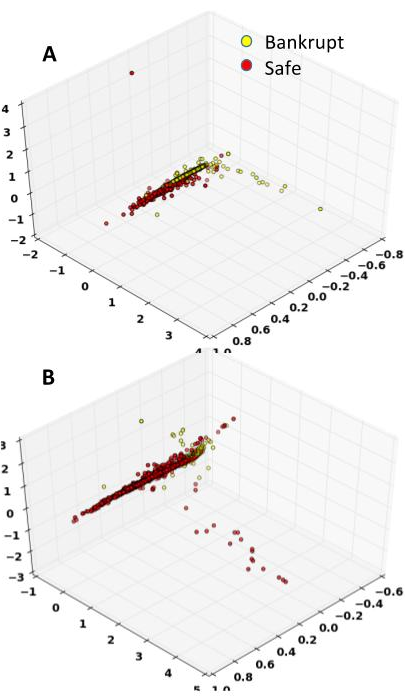
\includegraphics[width=81mm]{pca.png}
\caption{First three principal components of Original and Generated data. Figure A shows the First three principal components of the original data. Figure B shows the First three principal components of the generated data.}
\label{fig:Data}
\end{figure}


Most classification algorithms will only perform optimally when the number of samples of each class is roughly the same. Highly skewed datasets, where the minority is heavily outnumbered by one or more classes, have proven to be a challenge while at the same time becoming increasingly common. One way of addressing this issue is by re-sampling the dataset as to offset this imbalance with the hope of arriving at a more robust and fair decision boundary than one would otherwise. 


The Polish companies dataset is highly skewed. The majority (safe) class is over $97\%$ in all the 5 dataset. To overcome the skew class problem we used Synthetic Minority Over-sampling Technique (SMOTE). We implement this using imbalanced-learn package of scikit-learn contrib \cite{JMLR:v18:16-365}. 

For sampling using SMOTE, we first split our original data in $80\%-20\%$ split. We use the $80\%$ for data generation and keep the $20\%$ for the validation of our network model. Figure~\ref{fig:Data}-A. shows the first three principal components of the original data and Figure~\ref{fig:Data}-B. shows the first three principal components of the generated data. 

To model the network, we try two different approach and then compare the results obtained from the two techniques. The first technique used for learning to predict if the company is safe or bankrupt was based on the Net2Net initialization technique \cite{net2net}, which performs learning in a sequential manner starting with small MLPs and then scaling the neural network up to a larger size in width and depth by using the previous smaller network as a teacher to the new larger student network. This approach avoids the usage of a very large initial network and then re-learning the entire network from scratch if the performance is not suitable. The scaling of the network is performed by initializing the student network with the weights of the teacher network and then widening or deepening it. Widening involves adding additional neurons to a layer. Deepening involves adding a new hidden layer to the network. The advantage of the method is that it ensures that the student network improves upon the teacher network. The second approach is to train a FCN using the conventional method using the best architecture we obtain for the Net2Net approach. We will then compare the results of the two approach based on the performance metric discussed in section \ref{sec:metric}.


%we propose to treat this problem as an anomaly detection problem instead of binary classification problem. Anomaly detection (also known as outlier detection) is the identification of items, events or observations which do not conform to an expected pattern or other items in a dataset. Typically the anomalous items will translate to some kind of problem such as bank fraud, a structural defect, medical problems or errors in a text or in this case bankruptcy. Anomalies are also referred to as outliers, novelties, noise, deviations and exceptions \cite{anomaly}. In machine learning based anomaly detection we train an algorithm and obtain a model which captures the non-anomalous behaviour in the data. While testing we check if the test data can be fitted with the trained model. All the inconsistencies in fitting while testing are flagged as anomalies \cite{sakurada2014anomaly}.

%We consider safe companies as negative class (class 0) and bankrupt companies as positive class (class 1). 

%In this paper, we implement anomaly detection applying dimensionality reduction using Auto Encoders.


%Describe the computational approach -- based obviously on neural networks -- that you took to tackle the problem.

